\chapter{Konzeption und Implementierung}

Das neue Konzept, das in diesem Kapitel erklärt wird, beinhaltet die Migration von Datenbanken von der alten webbasierten Software zur neuen Software, die auf Umbraco CMS basiert. Die Funktionalitäten müssen gleichbleiben. Das Projekt ist in zwei große Pakete unterteilt – Paket A und Paket B. Im ersten Paket wird die Verwaltung des Frontend aufgebaut. Das Ziel ist es, maximale Flexibilität für den Website-Besitzer herzustellen und diesem zu ermöglichen, durch einfache Tätigkeiten bestimmte Zwecke zu erfüllen. In diesem Bereich soll der Inhalt der Webseite editiert, geändert und erweitert werden können. Umbraco verfügt über sogenannte „Grids“, die dazu dienen, das Design der Seite zu manipulieren und die bereits besprochenen Möglichkeiten auszunutzen. Dazu werden eigene Makros benutzt, in die ein Quellcode der SHOP-Komponenten hineingeschrieben wird. Somit kann der Auftraggeber Makros in beliebigen Teilen der Seiten einfügen. Umbraco-Forms werden als Formulare benutzt, damit der Nutzer die Felder selbst anordnen kann. Beide Pakete werden als Startknoten aus einer Umbraco-Instanz heraus verwaltet. Paket B ist als Kern der Seite aufgebaut und entspricht dem Online-Bestellsystem. Hier ist es wichtig, dass eine unkompliziert und reibungslos bedienbare, flexible Umgebung aufgebaut wird. Das System besteht aus drei Hauptkernen:
 
\begin{itemize}	
	\item Bestellsystem
	\subitem Kundenverwaltung (Anmeldung, Kundenbereich, Kommunikation)
	\subitem Artikelverwaltung
	\subitem Auftragsverwaltung
	\item E-Mail-Verwaltung
	\subitem E-Mail-Vorlagen anlegen, editieren, löschen
	\item Umsatzerfassung
	\subitem Umsatzübersicht nach Monat und Jahr
\end{itemize}

\section{Aufbau vom Umbraco}

Wie oben bereits erklärt wurde, ist Umbraco \cite{Wahlberg2011} ein Content-Management-System, das flexibel und benutzerfreundlich ist. Um die Funktionen besser verständlich zu machen, wird es in diesem Unterkapitel erläutert.
Das User Interface von Umbraco ist in drei Teile unterteilt. Der erste Teil ist die Hauptfunktion bzw. Section. Dort befinden sich die Hauptoptionen: Content, Media, Settings, Developer, Users, Members, Forms. Damit zwischen „Member“ und „User“ eindeutig unterschieden werden kann, werden die beiden Begriffe erklärt. „User“ ist jemand, der Zugriff zum „Umbraco-Backoffice“ und dort wiederum bestimmte Rechte hat.
Ein „Member“ wird von Umbraco für die Registrierung und Authentifizierung eines externen Besuchers benutzt. Das sind Personen, die nur das Frontend benutzen dürfen. Es kann auch eine „Custom Section“ erstellt werden, die im einem weiteren Unterkapitel erklärt wird. 

Der nächste Teil ist die Unternavigation oder auch Tree genannt. Dort stehen alle Unteroptionen, wobei jede Hauptfunktion ihre eigenen Unteroptionen hat. Im Folgenden werden die zugehörigen Funktionalitäten der Unteroptionen (Trees) betrachtet. Die Abbildung \ref{fig:UmbracoFunktionalitaet} stellt das Funktionsprinzip von Umbraco \cite{UmbracoHQ2018Backofficeoverview} dar.

\begin{figure}[h]
	\centering
	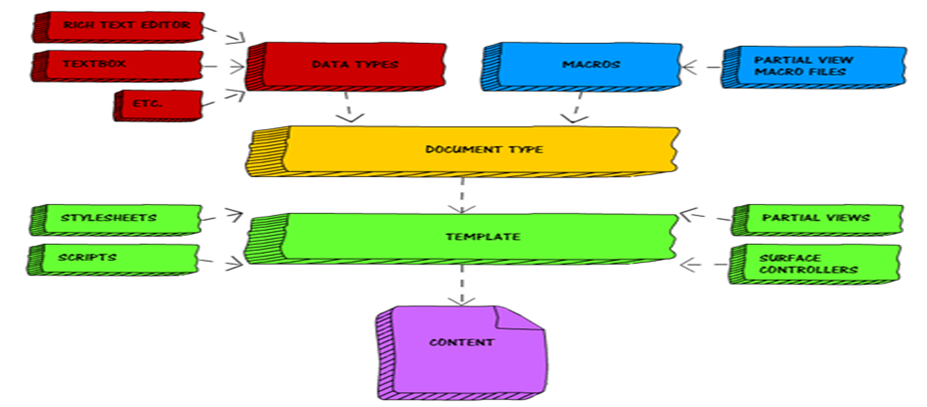
\includegraphics[width=1\linewidth]{Graphics/umbracoAufbau.png}
	\caption[Umbraco Backoffice]{Funktionalität vom Umbraco-Backoffice}\cite{droombiz2018}
	\label{fig:UmbracoFunktionalitaet}
\end{figure} 

\begin{itemize}	
	\item\textbf{Trees vom Content-Section:} In diesem Tree befinden sich alle Seiten, die im Website-Frontend erscheinen können. Dort befindet sich auch der Recycle Bin oder Papierkorb. Damit lässt sich die gelöschte Seite zurücksetzen.
	\item\textbf{Trees von der Media-Section:} Hier stehen alle hochgeladen Videos und Bilder zur Verfügung.
	\item\textbf{Trees vom Settings-Section:} In diesem Tree befinden sich CSS, JavaStript, Document Types und zugehörige Templates. PatialView ist auch dort, das eine Übertragungsfunktion von Backend zum Frontend hat.
	\item\textbf{Trees vom Developer-Section:} Hier stehen Trees zur Verfügung, durch die der Entwickler bereits erstellte Seiten weiter entwickeln kann. Das wird durch Data Typ, Macros, Packages, Relation Types, XSLT Files und Partial View Macro Files ermöglicht.
	\item\textbf{Trees vom User:}In diesem Bereich stehen die Benutzer, die mit bestimmtem Rechten das Umbraco-Backend benutzen dürfen. Für einen bestimmten User können verschiedene Rechte freigegeben werden. 
	\item\textbf{Trees vom Member-Section:} Hier sind Benutzer, die Frontend benutzen dürfen.
	\item\textbf{Trees vom Forms-Section: } Hier lassen sich verschiedene Arten von Formularen erstellen.
\end{itemize}

Der dritte Teil des Umbraco-Backoffice ist der Editierbereich. Dort werden alle Eigenschaften der jeweiligen Tree-Optionen dargestellt.

In der Abbildung \ref{fig:UmbracoBackoffice} wird gezeigt, wie das Umbraco-Backoffice aussieht.
\begin{figure}[h]
	\centering
	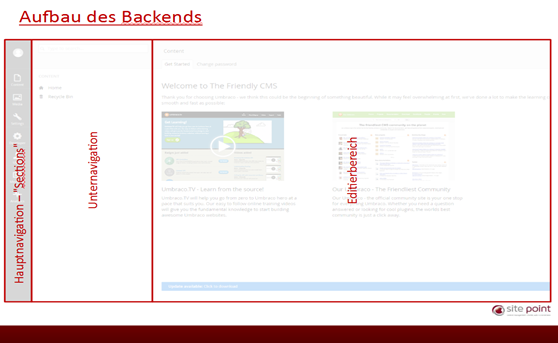
\includegraphics[width=1\linewidth]{Graphics/UmbracoBackend.png}
	\caption[Umbraco Backoffice]{Übersicht vom Umbraco-Backoffice}\cite{Beckert2017}
	\label{fig:UmbracoBackoffice}
\end{figure}

\pagebreak
\section{Paket A}

Damit der Auftraggeber mehr Flexibilität erhält, um die Frontend-Seite zu editieren, werden „Grids“ (Rahmen) verwendet. Ein Grid enthält zwölf Spalten, wobei diese auch verbunden werden können. So ist es möglich, dass die Seite beliebig aufgeteilt wird, wie in Abbildung \ref{fig:GridsLayout} gezeigt wird.

\begin{figure}[h]
	\centering
	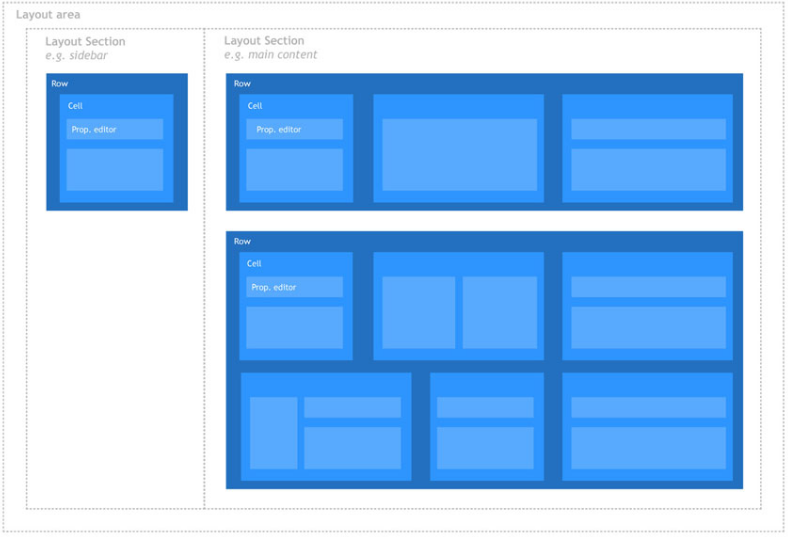
\includegraphics[width=1\linewidth]{Graphics/GridsLayout.png}
	\caption[GridsLayout]{Übersicht vom Umbraco-Grids}
	\label{fig:GridsLayout}
\end{figure}


Im Grid lassen sich eigene Einstellungen vornehmen. In dieser Arbeit werden zwei Beispielen gezeigt, wie Grids verwendet werden könnten, so etwa um die Farbe und die Größe der Schrift zu ändern. Für das geforderte Ziel werden der Rich Text Editor und Makros verwendet. Diese können im Rich Text Editor implementiert werden. Das soll in einem späteren Kapitel gezeigt werden. Hier werden nur die bereits erwähnten Beispiele betrachtet. Sie werden in den „Stylesheets“ unter „rte“ eingegeben. In Abbildung  \ref{fig:StylingGrind} wird gezeigt, wie CSS-Befehle in Umbraco geschrieben werden können.
     
     \begin{figure}[h]
     	\centering
     	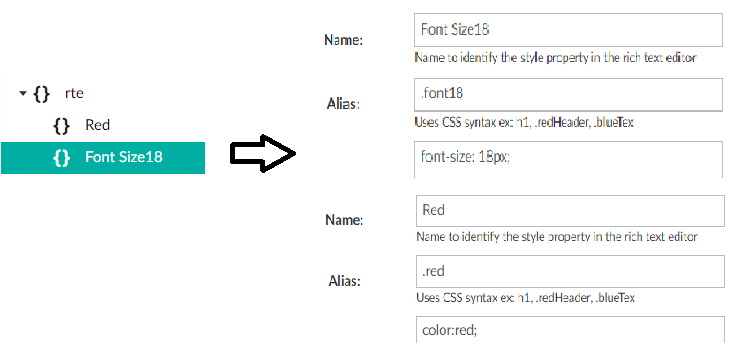
\includegraphics[width=0.6\linewidth]{Graphics/StylingGrind.png}
     	\caption[StylingGrind]{Styling vom Umbraco-Grids}
     	\label{fig:StylingGrind}
     \end{figure}
     
Über den Rich Text Editor kann der Inhalt des Frontend ebenfalls editiert werden, aber nur mit festen Optionen. Diese Stylesheets sind in den Rich Text Editor integrierbar, wodurch der Auftraggeber die Schriftart und die Farbe ändern kann. In der Abbildung  \ref{fig:schriftManip} wurde die Schrift auf rote Farbe und die Größe 18 pt geändert.

 \begin{figure}[h]
	\centering
	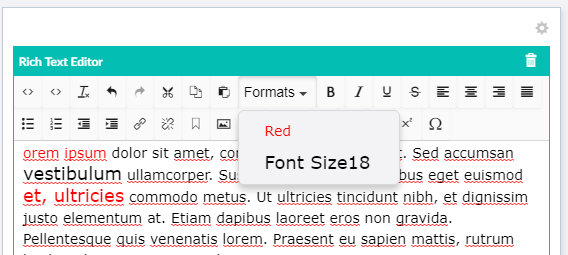
\includegraphics[width=0.6\linewidth]{Graphics/schriftManip.png}
	\caption[StylingGrind]{Styling in Umbraco-Grids - Rich text editor}
	\label{fig:schriftManip}
\end{figure}

\section{Paket B}

\subsection{Kundenverwaltung}
Die Kundenverwaltung umfasst den Bereich, der sich auf die Kunden bezieht.

Mehr wird im nächsten Unterkapitel erklärt.

\subsubsection{Kundenerfassung}

1.	Die vorgegebenen Bedingungen für diesen Bereich umfassen Registrierung und Anmeldung. Nach wie vor kann sich der Kunde anhand einer \ac{PIN} und seiner E-Mail-Adresse zu dem System anmelden. Diese PIN wird automatisch generiert und nach einer Bestätigung an die E-Mail-Adresse des Kunden gesendet. Dabei ist zu beachten, dass überprüft wird, ob sich die E-Mail-Adresse bereits in dem Register befindet. Außerdem wird gefordert, dass der Auftraggeber den Antrag des Kunden bestätigen kann. Nach der Bestätigung kann sich der Kunde anmelden und dort seine private Seite des Websystems verwalten. Die Funktionalitäten bleiben die gleichen wie bei dem alten System. Die Kundenerfassung wird durch Member-\ac{API} von Umbraco realisiert. Über „MemberService“ ist die MemberAPI erreichbar. Diese Bibliothek wird unter den Services \cite{UmbracoHQ2018Services} property von dem SurfaceController \cite{UmbracoHQ2018Models} zu Verfügung gestellt. Das ist eine komplexe Methode, für die verschiedene Dateien benötigt werden: (Controller, Model \cite{UmbracoHQ2018Models}, Partial View und Source Datei, in der View-Methoden über eine Aufruf-Funktion aufgerufen werden). Die zur Registrierung benötigte Information findet sich in der Model-Datei. Dort stehen die Model Properties oder auch die Parameter, mit denen hier gearbeitet wird. Über das Model werden die Properties von Partial View zum SurfaceController oder umgekehrt übertragen. Der SurfaceController ist gewissermaßen die ‚Autobahn‘ zur Umbraco-Datei, ein \ac{MVC}, der mit Umbraco interagiert. Er wird von der Bibliothek Umbraco.Web.Mvc.SurfaceController geerbt. Über Partial View werden die Verbindungen zwischen dem Kontakt-Formular und den Model Properties hergestellt. Hier handelt es sich eigentlich um eine Teilansicht, die vom Umbraco-Frontend benutzt wird. Dort befindet sich das Umbraco \ac{UI}. Die folgende Abbildung \ref{fig:Registrierung} zeigt, wie die obengenannten Begriffe sich zueinander verhalten.

\begin{figure}[h]
	\centering
	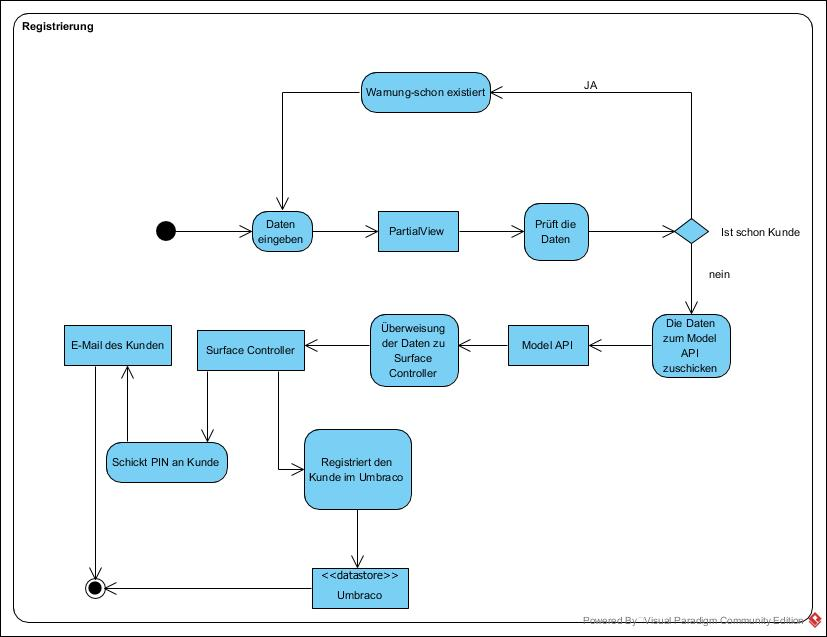
\includegraphics[width=1\linewidth]{Graphics/Registrierung.JPG}
	\caption[neues Konzept: Registrierung]{Neues Konzept zum Registrieren}
	\label{fig:Registrierung}
\end{figure}

Diese Möglichkeiten vom Umbraco erlauben dem Benutzer, sich leicht und bequem beim Server anzumelden oder sich zu registrieren. In Anhang - Kundenerfassung wird noch einmal übersichtlich gezeigt, wie genau vorzugehen ist, damit diese Anforderung erfüllt wird.


\subsubsection{Kundeansicht}

Um dem Kunden die Handhabung zu erleichtern, sollen folgende Möglichkeiten zur Verfügung stehen:

\begin{itemize}	
	\item Neue Bestellungen abgeben, aktuelle und vorherige Bestellungen ansehen
	\item Neue Nachricht schreiben und alte Nachrichten ansehen.
	\item Wichtige Information zu beachten
	\item Individuelle Information vom Auftraggeber.
\end{itemize}
1. Der Kunde bekommt einen PIN an seinem E-Mail. Die Listing \ref{lst:PINgenerator} und Anhang \ref{lst:EmailSchicken} zeigen, wie der Kunde seinen PIN bekommt, obwohl er sie bei der Registrierung nicht eingegeben hat.

\begin{lstlisting}[caption={JavaScript PIN Generator}, label=lst:PINgenerator]
function myFunction() {
document.getElementById('newInput').setAttribute('Value', Math.floor((Math.random() * 9000) + 1000));
}window.onload = myFunction;
\end{lstlisting}


2. 2.	Nach der Registrierung sieht der Kunde eine neue Seite. Dort kann er die obengenannten Optionen verwenden. Wenn der Kunde eine neue Bestellung tätigen will, wird ein neues Fenster geöffnet, in dem er die gewünschten Artikel wählen und bestellen kann. Die gewählten Produkte werden in den Datenbanken gespeichert, wo sie als vergangene Bestellungen verwendet werden können. Das selben Prinzip steht auch für die Kommunikation zwischen dem Auftraggeber und dem Kunden zur Verfügung. Wenn eine Nachricht geschrieben wird, wird sie in einer anderen Datenbank gespeichert. Vom Umbraco wird die Information direkt an den Kunden gesendet. Der Auftraggeber und der Kunde können in der Datenbank die Bestellungen und die Nachfragen ansehen. In den folgenden Kapiteln wird detailliert erklärt, wie die Kommunikation und die Aufträge funktionieren. 
3.Wie gefordert, wird dem Kunde eine Profile-Seite über Member angezeigt. Das bedeutet, dass diese Seite für den jeweiligen Kunden personalisiert ist. Die Abbildung wird über memberId geschehen. Es wird ein Filter erstellt, durch den sich diese Personalisierung herstellen lässt. memberId befindet sich in der Umbraco-Member-Datenbank. Mithilfe von Macros und Grids wird die Kundeansicht entwickelt. 
Das, was im Kundenansicht gemacht wurde, ist Verwendung von Macros und Grids. (zur Veranschaulichung siehe Abbildung  \ref{fig:kundenansichtNew}). 

\begin{figure}[h]
	\centering
	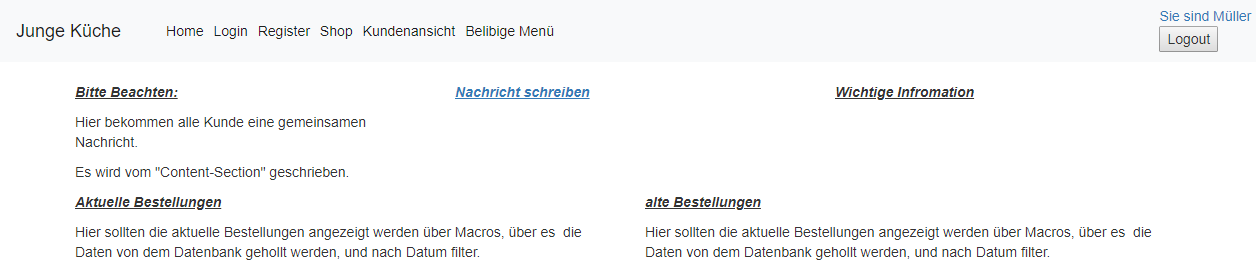
\includegraphics[width=1\linewidth]{Graphics/kundenansichtNew.png}
	\caption[Kundeansicht]{Kundeansicht}
	\label{fig:kundenansichtNew}
\end{figure}

Über ein Makro wie in Listing \ref{lst:macroKundenansicht} ist es möglich, die Meldungen vom Auftraggeber unter „Wichtige Information“ zu sehen. Im Makro wurde eine Methode geschrieben, über die die Übertagung von der Member-Section zur Content-Section ermöglicht wird. Abbildung \ref{fig:kundenansichtNew} zeigt, wie der Auftraggeber dem Kunden eine Informationsmeldung aus dem Member-Bereich schickt.

\begin{figure}[h]
	\centering
	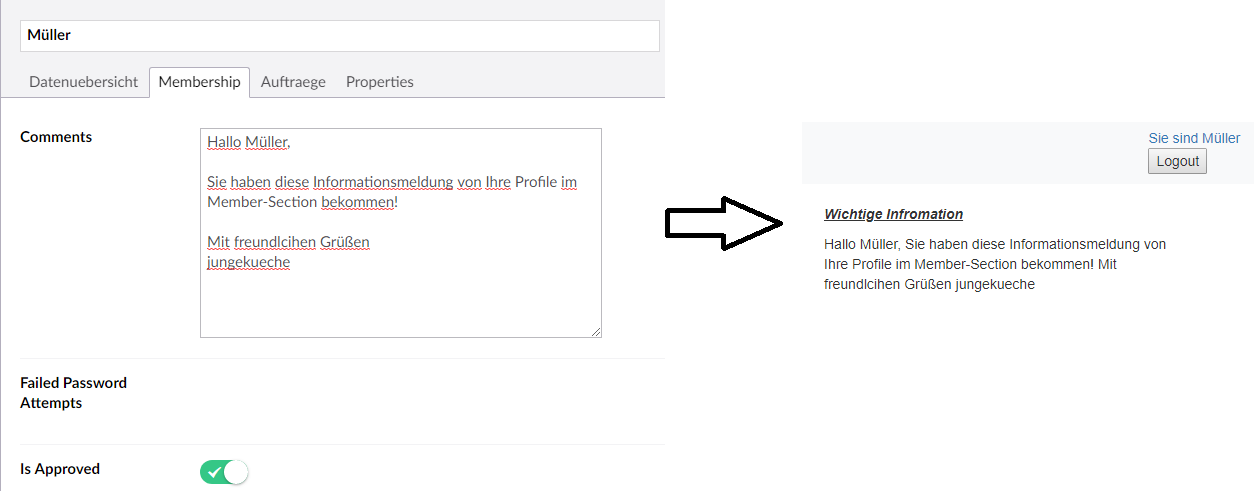
\includegraphics[width=1\linewidth]{Graphics/kundenAnsichtWichtInf.png}
	\caption[Kundeansicht]{Übertragung der Informationsmeldung von Member-Section zu Kundenansicht}
	\label{fig:kundenAnsichtWichtInf}
\end{figure}
\pagebreak
\begin{lstlisting}[caption={Macro zum Kundenansicht}, label=lst:macroKundenansicht]

@inherits Umbraco.Web.Macros.PartialViewMacroPage


@{
	var memberID = ApplicationContext.Current.Services.MemberService.GetByUsername(Membership.GetUser().UserName);
	var info = memberID.Comments;
}
@info
\end{lstlisting}

Das Kontaktfenster und allgemein die Bestellungen werden im weiteren Unterkapitel erläutert. Das gesamte Bild wird im Abbildung \ref{fig:KundenansichtNeu} dargestellt.

\begin{figure}[h]
	\centering
	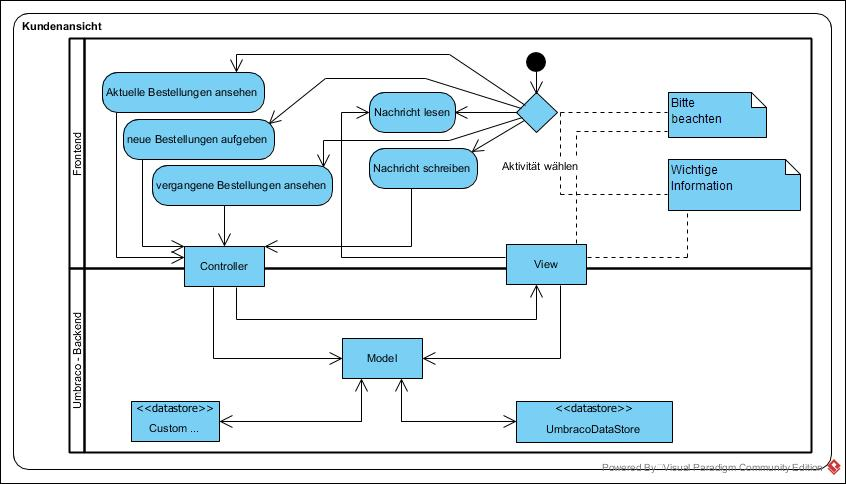
\includegraphics[width=1\linewidth]{Graphics/KundenansichtNeu.jpg}
	\caption[Funktionalität von Kundenansicht]{Funktionalität von Kundenansicht}
	\label{fig:KundenansichtNeu}
\end{figure}

\subsubsection{Auftraggeberansicht}
  
1.	Mithilfe der Umbraco-Member-Section kann der Auftraggeber seine Kunden filtern, nach dem Name suchen oder löschen, etwa nach vorgegebenen Einstellungen wie ListView\cite{UmbracoTV2018ListView}. Es können auch zusätzliche Properties erstellt werden. Diese lassen sich können über ein Extra-Attribut in der Model-Datei mit dem Frontend verbinden. Hier werden die neuen Tabs und Properties erstellt. Als Beispiel wird hier die Tab-„Datenuebersicht“ gezeigt. Dort befindet sich eine Property „Ort“. Im Tab-Membership ist „Password“ ein zusätzliches Beispiel. Davon können mehrere eingebaut werden. Die Abbildung \ref{fig:auftraggeberAnsichtDaten} zeigt diesen Tab und die zugehörige Property dar.  

\begin{figure}[h]
	\centering
	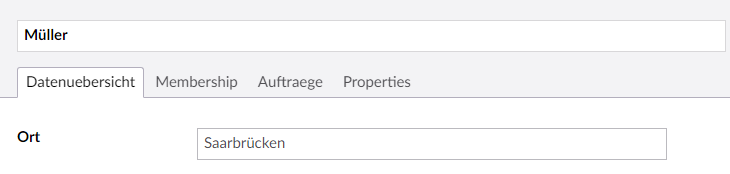
\includegraphics[width=1\linewidth]{Graphics/auftraggeberAnsichtDaten.png}
	\caption[Kundeansicht]{Beispiel zur Erstellung eines extra Tab und Property}
	\label{fig:auftraggeberAnsichtDaten}
\end{figure}
 Wie bereits erläutert wurde, wurde ein Macro erstellt, durch das die Information zum jeweiligen Kunde zugehörig ist. 

Wie bereits erläutert, wurde ein Makro erstellt, durch das die Information dem jeweiligen Kunden zugeordnet ist.
Um die Migration problemlos durchführen zu können, muss eine neue Zuordnung im Member-Bereich hergestellt werden. Die neuen Properties müssen mit den alten übertragenen Attributen der Member-Datenbank übereinstimmen. Dies wird im Unterkapitel „Übersicht“ erläutert.

\subsubsection{Kommunikation}

In diesem Kapitel wird die Kommunikation zwischen dem Auftraggeber und dem Kunden beschrieben. Als Anforderung wird eine übersichtliche Kommunikationsmethode mit Filtern (gelesen, nach Kunden suchen etc.) festgestellt.

Dafür wird eine ContentAPI \cite{UmbracoHQContent2018} verwendet. In der Kundenansicht kann der Kunde über ein View-Nachricht-Formular Nachrichten verschicken. Mithilfe des Models und des SurfaceController wird die Nachricht in der Umbraco-Content-Section erstellt. Dort wird sie als neue Untertreenode im vorgesehenen Tree „Nachrichten“ positioniert. Dieser Tree wird mithilfe von Umbraco-ListView modelliert. Umbraco-ListView ermöglicht beliebig viele Untertreenodes, die in einem einzigen Tree gelagert werden. Um die Nachrichten dem zugehörigen Kunden zuzuordnen, wird in die jeweilige Nachricht die IdNummer des Kunden integriert. Mithilfe dieser Nummer kann auch ein Filter erstellt werden.
Somit kann die Kunde nur seine privaten Nachrichten lesen. Das Listing \ref{lst:NachrichController} und die Abbildungen \ref{fig:NachrichtNEU} und \ref{fig:NachrichtUmbraco} zeigen den Verlauf der Kommunikation.

\begin{figure}[h]
	\centering
	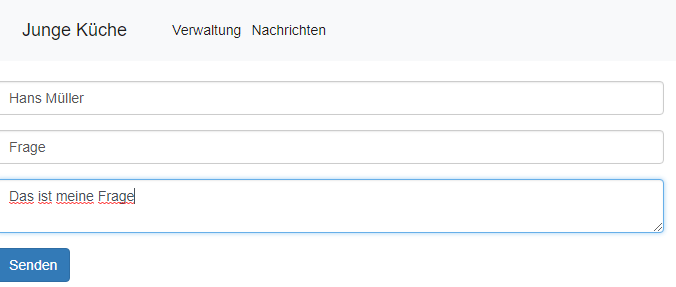
\includegraphics[width=0.7\linewidth]{Graphics/NachrichtNEU.png}
	\caption[Nachricht Formular]{Nachricht Formular}
	\label{fig:NachrichtNEU}
\end{figure}
\begin{lstlisting}[caption={NachrichController}, label=lst:NachrichController]

namespace newKonzept.Controllers.NachrichtController
{
public class NachrichtController : SurfaceController
{
// GET: Nachricht
public ActionResult Index()
{
return PartialView("NachrichtPartial/NachrichtPartial", new NachrichtModel());
}
[HttpPost]
public ActionResult HandleFormSubmit(NachrichtModel model)
{
if (!ModelState.IsValid)
{
return CurrentUmbracoPage();
}

var memberID = ApplicationContext.Current.Services.MemberService.GetByUsername(Membership.GetUser().UserName);
model.SenderId = memberID.Id;
var comment = Services.ContentService.CreateContentWithIdentity(model.Sender, CurrentPage.Id, "nachricht");

comment.SetValue("Betreff", model.Betreff);
comment.SetValue("Sender", model.Sender);
comment.SetValue("Message", model.Message);
comment.SetValue("SenderId", model.SenderId);

Services.ContentService.Save(comment);

Services.ContentService.Save(comment);
TempData["success"] = true;

return RedirectToCurrentUmbracoPage();
}
}
}
\end{lstlisting}


\begin{figure}[h]
	\centering
	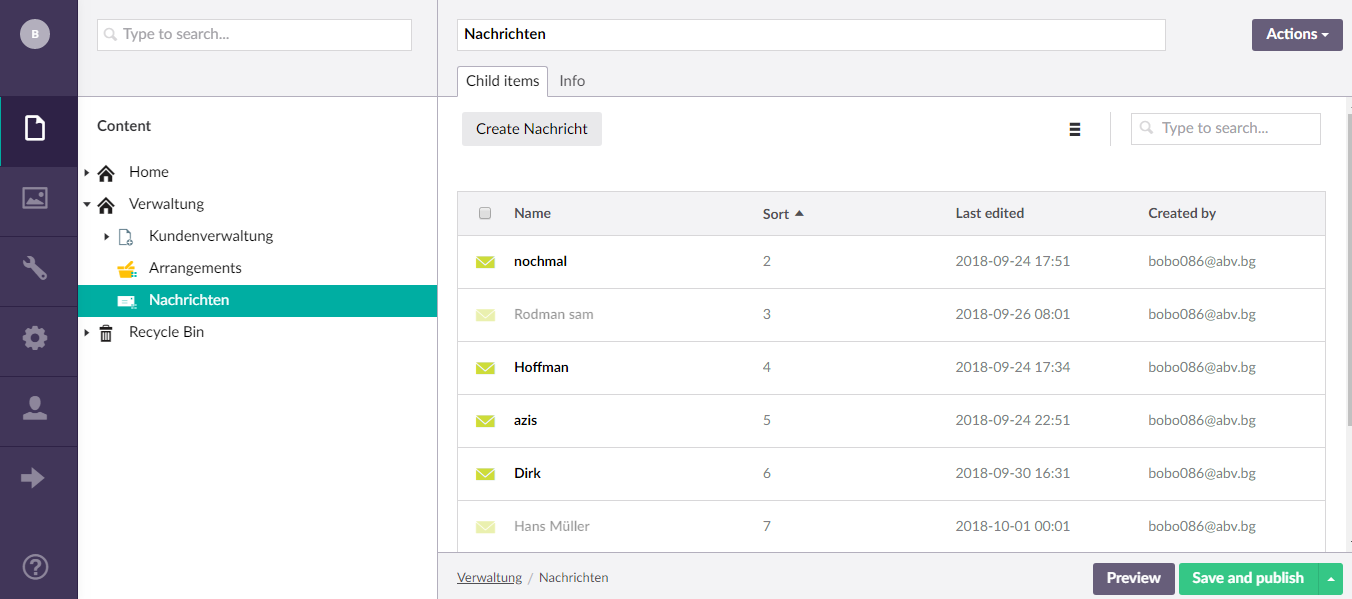
\includegraphics[width=0.7\linewidth]{Graphics/NachrichtUmbraco.png}
	\caption[NachrichtUmbraco]{Nachricht in Umbraco-Backoffice}
	\label{fig:NachrichtUmbraco}
\end{figure}

Wenn die Nachricht noch nicht gelesen wurde, ist sie hellgrau markiert In dem geöffneten Fenster wird die gesendete Nachricht angezeigt. Daneben befindet sich das „Antwort“-Tab, über das der Auftraggeber die Frage beantworten kann. Die Nachrichten werden nach memberID gefiltert. In den Abbildungen \ref{fig:Message} und \ref{fig:antwort} wird die Rückfrage dargestellt.

\begin{figure}[h]
	\centering
	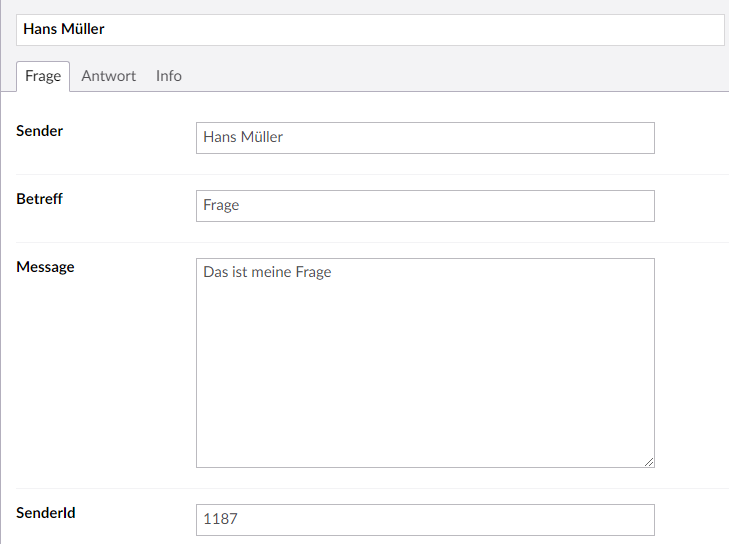
\includegraphics[width=0.7\linewidth]{Graphics/Message.png}
	\caption[Nachricht]{Die Nachricht gelesen}
	\label{fig:Message}
\end{figure}

\begin{figure}[h]
	\centering
	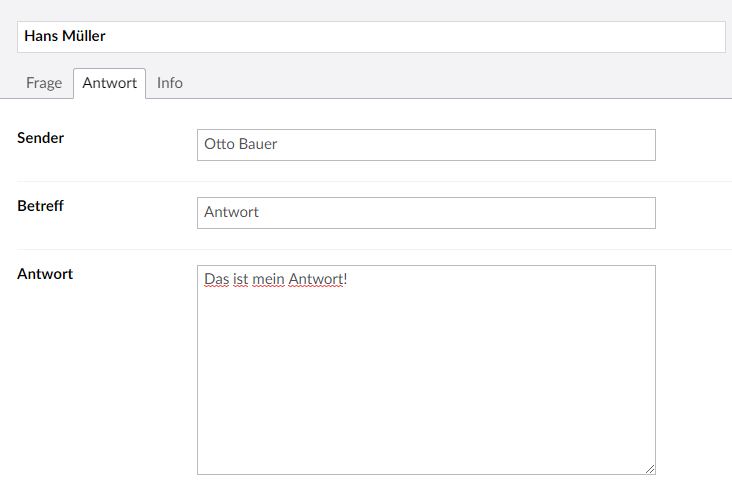
\includegraphics[width=0.7\linewidth]{Graphics/antwortMassege.png}
	\caption[Nachricht]{Antwort Schreiben}
	\label{fig:antwort}
\end{figure}

\pagebreak

Im Listing \ref{lst:NachrichFilter} ist der Filter, der in einem Macro integriert wird, dargestellt.

\begin{lstlisting}[caption={NachrichFilter}, label=lst:NachrichFilter]

<ul>

@foreach(var item in selection){

var pageId = item.GetPropertyValue
<string>
("senderId");
if(pageId.ToString() == memberID.Id.ToString()){
<li>
<a href="@item.Url">@item.Name</a>
</li>
}
}
</ul>
\end{lstlisting}

Der Kunde sieht die Antwort von dem Auftraggeber, wie in der Abbildungen \ref{fig:bekommen} und \ref{fig:alleNachrichten} gezeigt.
\begin{figure}[h]
	\centering
	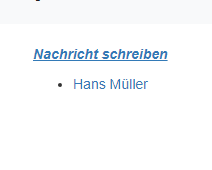
\includegraphics[width=0.3\linewidth]{Graphics/nachrichtBekomm.png}
	\caption[Nachricht]{Antwort erhalten}
	\label{fig:bekommen}
\end{figure}

\begin{figure}[h]
	\centering
	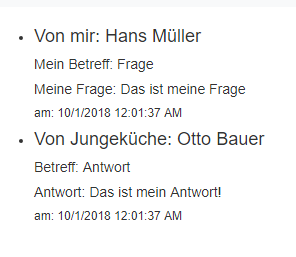
\includegraphics[width=0.3\linewidth]{Graphics/dialog.png}
	\caption[Nachricht]{Alle Nachrichten}
	\label{fig:alleNachrichten}
\end{figure}
 
 \pagebreak
 
\subsection{Artikelverwaltung}

\subsubsection{Erfassen, editieren und löschen}

Nach der vorgegebenen Aufgabe muss der Online-Editor zwei Kategorien enthalten – Arrangements und Artikel-Standard. Diese müssen mit den zugehörigen Webseiten gekoppelt werden. Eine Anforderung lautet, dass die Artikel-Verwaltung einfach funktionieren muss und die Artikel, die sich in der Webseite befinden, direkt mit den Artikeln, die in der Umbraco-Content-Section stehen, gekoppelt sein müssen. Auf der alten Seite ist die Artikel-Verwaltung nicht mit den zugehörigen Seiten gekoppelt. Die Migration der Artikel ist nicht gefordert.

Das entsprechende Ziel wird über Makros, die PetaPoco-Datenbank \cite{Robinson2018} und die von Umbraco vorgegebenen Funktionen erreicht. Zuerst wird Umbraco ListView verwendet, damit sich die erstellten Artikel in der Umbraco-Content-Section unter einer gemeinsamen Unteroption befinden. Außerdem ist vorgegeben, dass die neu erstellten Artikel direkt editiert werden können. Abbildung \ref{fig:ArtikelVerwaltung} zeigt, wie die Artikel-Verwaltung aussieht.

\begin{figure}[h]
	\centering
	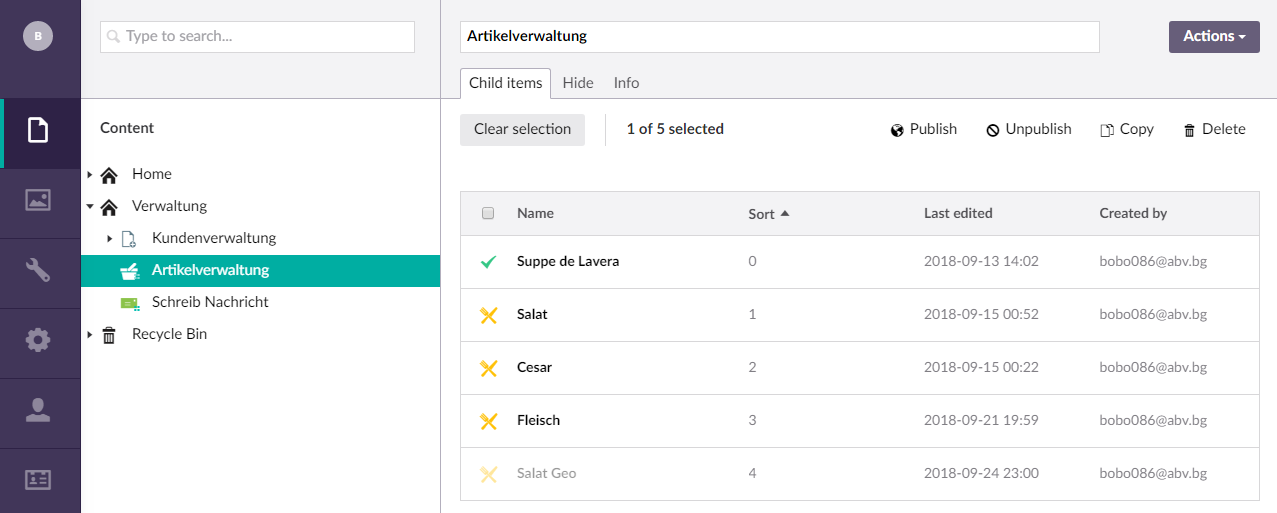
\includegraphics[width=1\linewidth]{Graphics/ArtikelVerwaltung.png}
	\caption[ArtikelVerwaltung]{Übersicht der Artikel-Verwaltung}
	\label{fig:ArtikelVerwaltung}
\end{figure}

Wenn der Artikel „unpublish“ ist, kann er nicht im Frontend verwendet werden. Wenn die Artikel bereits erstellt wurden, wird ein Quellcode im Makro programmiert. Dieses Makro wird in das oben erwähnte Grid integriert. Dadurch wird der Inhalt der Artikel zum Frontend übertragen. Der Inhalt wird nicht nur mit den Webseiten, sondern auch mit dem Shop-Menü gekoppelt. Damit erhält der Auftraggeber mehr Selbständigkeit. In der nächsten Abbildung wird gezeigt, wie mit der Erstellung eines Artikels seine Daten sowohl an die zugehörige Seite als auch an das Shop-Menü gekoppelt werden. Wenn der Kunde registriert ist, kann er die von dem Auftraggeber eingegebenen Artikelaus dem Shop wählen. Nach der Bestellung werden die Daten in der Datenbank „Artikel“ gespeichert. Gleichzeitig werden diese Daten zusammen mit den Kunden-Daten auch in der Datenbank „Auftraege“ gespeichert. In Abbildung \ref{fig:Shop} ist zu sehen, dass die Daten der Artikelverwaltung erfolgreich zum Shop gesendet wurden.


\begin{figure}[h]
	\centering
	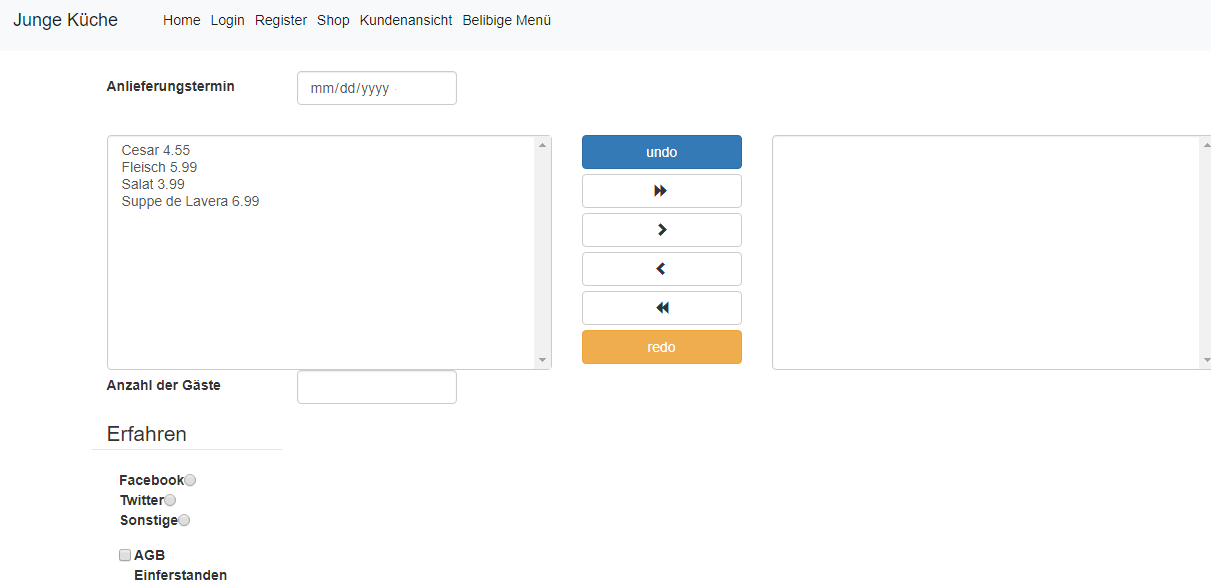
\includegraphics[width=1\linewidth]{Graphics/shop.png}
	\caption[Shop]{Übersicht des Shops}
	\label{fig:Shop}
\end{figure}


\subsection{Auftragsverwaltung}

\subsubsection{Übersicht}

Das vorgegebene Ziel ist eine Übersicht über die Aufträge und Nachrichten. Diese An-sicht soll in einer eigenen Umbraco-Section umgesetzt werden. Die Artikeldatenbank soll von Access nach SQL transportiert werden. Es muss eine neue Zuordnung zu Umbraco-Member geben.
Das vorgeschlagene Konzept umfasst die Migration der Access-Datenbankdatei und die Erstellung einer neuen Custom-Section.

1.	Um eine neue Section aufzubauen, wird zunächst eine Klasse-Datei benötigt, mit der Methoden aus den Bibliotheken „umbraco.buisnesslogic“ und „umbraco.interfaces“ aufgerufen werden. Über die „Application“-Methode und das „IApplication“-Interface wird die Custom-Section erstellt. Danach  wird die Übersicht über den AngularJS-Controller und HTML erstellt. Diese Dateien werden zum API-Controller über das Paket-Manifest referenziert. In diesem Controller werden die eigentlichen Funktionalitäten der Custom-Section realisiert. Mithilfe des API-UmbracoAuthorizedJsonController werden die Daten über die Model-Attribute der bereits erstellten und im vorherigen Unterkapitel erwähnten Datenbank „Auftraege“ zur Verfügung gestellt. Die Datenbanken werden über PetaPoco erstellt. In der Abbildung \ref{fig:CustomSection} wird die Kommunikation gezeigt.
 
 \begin{figure}[h]
 	\centering
 	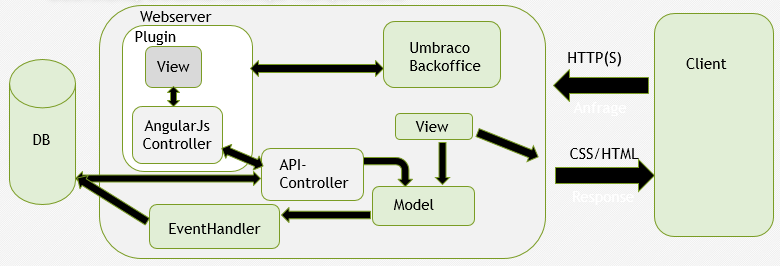
\includegraphics[width=1\linewidth]{Graphics/CustomSection.png}
 	\caption[Shop]{Eine Übersicht von Kommunikation zwischen verschiedene Elemente}
 	\label{fig:CustomSection}
 \end{figure}
 
2.	Wie gefordert, soll eine Migration der Access-Datenbank zu Umbraco durchgeführt werden. Das angestrebte Ziel ist, dass die alten Daten in der neuen zugehörigen Datenbank gespeichert werden. Die neuen betrachteten Datenbanken sind Custom-„Artikel“ und „Umbraco-Member“. Nach grundlegender Recherche wurde ein Konzept erstellt. Grundsätzlich stehen in der Umbraco-Member-Section \cite{OurUmbraco2018} drei Unteroptionen zur Verfügung – Members, Member Types und Member Groups. In Member Type werden die Einstellungen (Properties) des Members aufgebaut. Dort wird ein neuer Member Type mit extra Properties erstellt. Das folgende Konzept geht davon aus, dass die Datenbanken von Access in CSV-Format konvertiert sind. Das bedeutet, dass die Access-Datenbankformat-Datei in eine Text-Datei umgewandelt wird und dann die Methode StreamReader genutzt werden kann. Um das vorgegebene Ziel zu realisieren, muss ein SurfaceController erstellt werden, der die Übertragung leitet. Umbraco verfügt über spezielle ‚Autobahnen‘, durch die es möglich ist, festgelegte Sections in Umbraco zu manipulieren. Diese werden „Services“ genannt und über ApplicationContext aufgerufen. In diesem Fall wird „MemberService“ genutzt. Damit die Datei gelesen werden kann, wird die Funktion StreamReader verwendet. Damit wird die gelesene Datei in einer Variablen gespeichert. Der Inhalt der Datei wird von diesen Variablen mithilfe von dem Befehl-split zu einem Array gespeichert. Jeder Teil des Array wird über MemberService-Befehle und -Methoden in Umbraco Members gespeichert. Im Anhang \ref{lst:migrationsController} ist der Quellcode nachzulesen und in der Abbildung \ref{fig:DBMigration} ein Schema zur Migration.

 \begin{figure}[h]
	\centering
	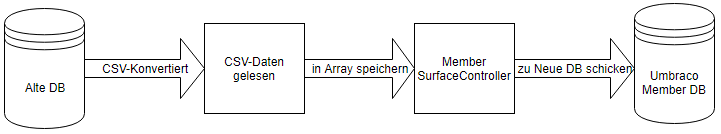
\includegraphics[width=1\linewidth]{Graphics/DBMigration.png}
	\caption[DatenbankMigration]{An neue Datenbank schicken}
	\label{fig:DBMigration}
\end{figure}

Wenn die Kundendaten schon übertragen wurden, kann dasselbe Prinzip der Migration für die Artikel verwendet werden. Hier wird als Ziel anstelle der MemberService- Datenbank die Artikel-Datenbank verwendet. Nach der Umwandlung der Access-Datenbankdatei in das CSV-Format wird diese Datei über die Methode StreamReader gelesen, danach wird die Information in einem Array gespeichert. Über den API-Controller werden die Daten in die Artikel-Datenbank übertragen. In Listing \ref{lst:DBInputArtikel} wird anschaulicher gezeigt, wie die Übertragung der Daten abläuft.

\begin{lstlisting}[caption={Datenbank "Artikel" - Transfer}, label=lst:DBInputArtikel]

var setArtikel = new Artikel();
var db = new PetaPoco.Database("umbracoDbDSN");
setArtikel.kundeID =_split[0];
setArtikel.bezeichnung = _split[1];
setArtikel.beschreibung = _split[2];
setArtikel.preis = _split[3];
setArtikel.art = _split[4];
setArtikel.kannWaehelen = m_split[5];

db.Insert(setArtikel);
\end{lstlisting}

\subsubsection{Detailansicht}

Hier wird gefordert, dass der Auftraggeber die Aufträge bearbeiten kann, den Status ändern, Positionen editieren, hinzufügen oder löschen, dem Kunden Freigaben erteilen (zum Beispiel das Aussuchen der Positionen) und eine Rechnungsnummer vergeben. Diese Aktivitäten sind dieselben wie auf der alten Webseite und müssen in einer eigenen Umbraco-Section umgesetzt werden.
Die Erstellung einer Custom-Section ist bereits bekannt. Hier wird sie mit der Auftraege- und der Member-Datenbank über AngularJS-Controller anhand des Package-Manifest mit dem API-UmbracoAuthorizedJsonController verbunden. In den Listings \ref{lst:AngularJS} und \ref{lst:API-Controller} wird gezeigt, wie die Daten aus der Datenbank aufgerufen werden.

\begin{lstlisting}[caption={AngularJS-Controller ruft die zugeordnete Methoden im API-Controller}, label=lst:AngularJS]

angular.module("umbraco").controller("Detailansicht.editController", function ($scope, $routeParams, auftragResource, navigationService, notificationsService) {

	$scope.loaded = false;

	// Inhalt wird geladen
	if ($routeParams.id == -1) {
		$scope.auftrag = {};
		$scope.loaded = true;
	}
	else {
	// Artikel wird geladen
		auftragResource.getById($routeParams.id).then(function (response) {
		$scope.auftrag = response.data;
		$scope.loaded = true;
		});
	}

	$scope.save = function (auftrag) {
		auftragResource.save(auftrag).then(function (response) {
		// $scope.auftrag.$isdirty = false;
			$scope.auftrag = response.data;
			notificationsService.success("Success", auftrag.auftragId + " " + " has been saved.");
			navigationService.syncTree({ tree: 'auftragTree', path: [-1, $scope.id], forceReload: true }).then(function (syncArgs) {
				navigationService.reloadNode(syncArgs.node);
				});
			});
	}
});
\end{lstlisting}

\begin{lstlisting}[caption={API-UmbracoAuthorizedJsonController}, label=lst:API-Controller]

namespace newKonzept.Controllers.DB
{
	[PluginController("Detailansicht")]
	public class AuftragApiController : UmbracoAuthorizedJsonController
	{
		private Database db = new Database("umbracoDbDSN");
		public IEnumerable<Auftraege> GetAll()
		{
			List<Auftraege> liste = new List<Auftraege>();
			foreach (Auftraege auftrag in db.Query<Auftraege>("SELECT * FROM Auftraege"))
			{
				liste.Add(auftrag);
			}
			return liste;
		}
	public Auftraege GetById(int id)
	{
		return db.SingleOrDefault<Auftraege>("SELECT * FROM Auftraege WHERE auftragId=@0", id);
	}

	public Auftraege PostSave(Auftraege auftrag)
	{
		if (ModelState.IsValid)
		{			
			if (auftrag.auftragId > 0)
			{
				db.Update(auftrag);
			}
			else
			{
				db.Insert(auftrag);
			}
		}
		return auftrag;
	}

	public int DeleteById(int id)
	{
		var db = new PetaPoco.Database("umbracoDbDSN");
		return db.Delete<Auftraege>("WHERE auftragId=@0", id);
	}
}
\end{lstlisting}

Die Daten aus der Member-Datenbank werden als String über MemberService aufgerufen und in ein Array gespeichert. Dieses Array wird von der AngularJS aufgerufen und an den HTML-Plugin-Editor geschickt. Die Daten des Members können in der Detailansicht nicht geändert werden, daher werden sie als String verwendet.